\chapter{应用筛选框架\mytool}
\label{chp:fakerevealer}

\mytool 是由Python 3开发的一个应用筛选框架,由\componentA 、\componentB 和\componentC 三个组件组成,\autoref{fig:FakeRevealer}展示了\mytool 的整体流程图。
输入初始正版应用的信息,\mytool 在经过迭代搜索、样本下载、应用过滤三个步骤之后,将以CSV文件和JSON文件的形式输出仿冒应用各数据项和拓展后的正版应用信息。

\begin{figure}[htbp]
	\centering
	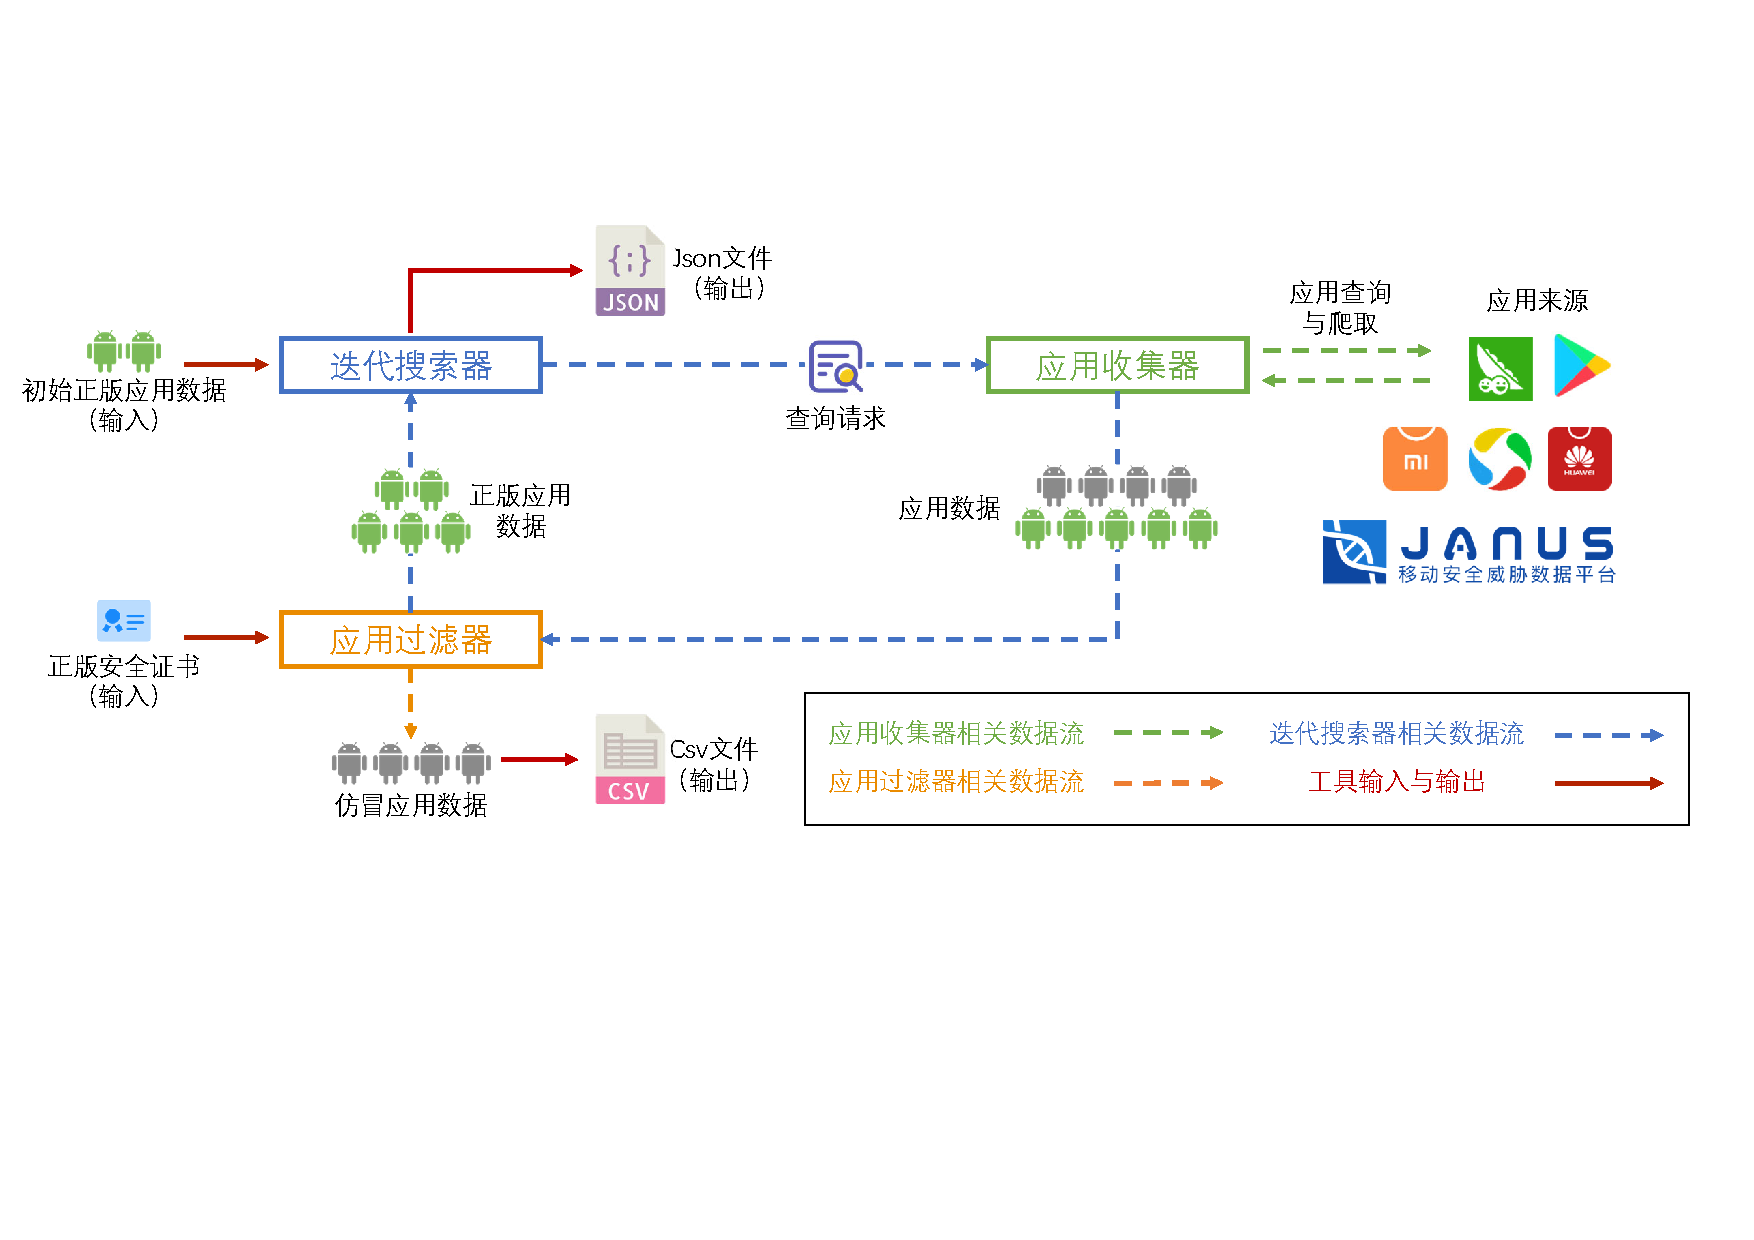
\includegraphics[width=\textwidth]{./Figures/edwin-fakerevealer}
	\caption{\mytool 整体结构}
	\label{fig:FakeRevealer}
	\vspace{-3mm}
\end{figure}


\section{组件设计与实现}


\subsection{\componentA }
\componentA 是与应用来源直接交互的部分,分为两个不同的子模块,分别是网络爬虫模块和APK包预处理模块。
在接收到应用收集请求之后,\componentA 会先根据收集请求,利用网络爬虫模块下载应用,然后再用APK包预处理模块对下载完毕的APK包提取信息,方便后续操作。

1)\ \emph{网络爬虫模块} \quad
本模块负责接收\componentA 的输入,根据输入中的需求从应用来源中查询并下载对应的App。
由于Janus平台上已经有提前收集好的源于各个应用市场的App样本,我们可以直接从Janus上爬取应用。

实际上,虽然应用商店提供应用查询、下载的API不同,不存在可以对应所有应用市场的爬虫脚本,但只要能分析出这些API的名称和用法,结合应用商店账户的Cookies,我们也能从商店中下载应用。
考虑到这个方面,我们开发了插件化的爬虫模块。
针对不同的应用商店,我们可以在使用网络包分析工具(如Burpsuite~\cite{burpsuite})解析到API与Cookies信息之后,将对应API和Cookies写入配置插件,再对网络爬虫模块配置对应当前商店的插件,开始爬取应用。

在具体实现方面,我们利用Python自带的urllib库实现对网络资源的访问;由于下载是可以并发进行的事务,为了能提高运行效率,我们利用了threading库对网络爬虫模块提供了多线程特性。

2)\ \emph{APK包预处理模块} \quad
这个模块负责从下载完毕的APK包中提取指定的数据项,存入键值对中,最后将所有应用的数据键值对以列表形式返回,作为\componentA 的输出。
APK文件中虽然包含着应用的所有信息,但我们的应用筛选并不需要用到整个APK文件,所以我们可以把筛选需要用到的数据先提取出来,后续处理时直接调用与该APK包有关的数据即可。
同时,由于不同APK包的大小不一,所需下载时长也各异,我们利用了较大的应用还在下载的时间,对已经下载完毕的APK提取信息。
比起让\componentA 直接返回下载完毕的APK包、待后续需要数据时再进行数据提取的方法,这样的设计可以减小内存占用,也提高了框架的运行效率。

具体实现方面,APK包预处理模块使用Python的os库实现对命令行指令的调用,然后利用Android SDK中自带的命令行工具aapt对APK包进行解析,获取指定的数据项。


\subsection{\componentB }
这个组件的设计利用了基于一个BFS的算法,详情可见\autoref{alg:bfs}。
根据缓存中的正版应用信息,本组件向\componentA 提交查询、下载样本的请求。
在利用\componentC 过滤获得的应用信息后,再根据其中正版应用的信息扩增缓存中的数据,进行下一轮迭代搜索。

\begin{algorithm}[!ht]
	\tablewuhao
	\caption{迭代搜索算法}
	\label{alg:bfs}
    \KwIn{ $targetItems$,列表,用于拓展的数据项}
    \KwIn{ $legalApkInfo$,列表,包含正版应用及其信息键值对}
	\KwOut{ $cache$,列表,缓存拓展后的正版应用信息键值对}
	\SetKwProg{Fn}{Function}{:}{}

	\Fn {iterSearcher($legalApkInfo, targetItems$)} {

        $wtQueue$ = $\emptyset$;

        $cache$ = $\emptyset$;

        \For {$apkInfo \in legalApkInfo$} {

            \For {$item \in targetItems$} {

                $wtQueue$.add(${item: apkInfo[item]}$);

            }

        }

    	\While {$wtQueue \ne \emptyset$} {

    		$key, val$ = $wtQueue$.pop();

    		\If{${key: val} \in cache$} {continue;}

    		$cache$.add(${key: val}$);

    		$newSamples \gets$ appRetriever($key, val$);

    		\For {$sample \in newSamples$} {

                $isLegal \gets $ FakeFilter($sample$).getResult();

    			\If {$isLegal$} {

    				$sampleInfo \gets sample$.getInfo();

    				\For {$item \in targetItems$} {

    					$wtQueue$.add(${item: sampleInfo[item]}$);

    				}

    			}

    		}

    	}

    \KwRet{$cache$};

    }

\end{algorithm}

\autoref{alg:bfs}的输入有两项,分别是已有的正版应用信息列表$legalAppInfo$和要用来拓展搜索范围的数据项$targetItems$。

算法开始前,我们先遍历每个正版应用的信息,将要每个要拓展搜索的数据项对应的内容$apkInfo[item]$插入到待查询队列$wtQueue$中,完成初始化(第4 - 6行)。
然后我们开始迭代搜索应用。
每次迭代中,我们都从$wtQueue$中取出一组键值对,其中键$key$为本次迭代中用于搜索新应用的数据项,$val$为数据项对应的值(第8行)。
取出键值对之后,我们先检查该键值对是否已经被用于之前的搜索中。
如果该键值对之前已经出现过,那么我们跳过本轮迭代,重新取一组键值对进行搜索;
否则,我们将本组键值对放入数据缓存$cache$,表示该组键值对已被使用过。
之后,我们将键值对传递给\componentA ,\componentA 会生成对应查询,从应用来源中获取数据项相关的应用(第12行)。
对于\componentA 返回的应用集$newSamples$中的每个样本$sample$,我们会用\componentC 检查$sample$是否为正版样本。
如果是正版样本,那么我们将从该样本中获取对应的数据$sampleInfo$,然后将其中与待拓展对应项$item$对应的内容插入到待查询队列$wtQueue$中(第15 - 18行)。
当应用集$newSamples$中的所有样本都被筛选检查过之后,本轮迭代结束。
如果$wtQueue$中的所有键值对都已经被检索完毕(即$wtQueue$为空),本算法流程结束,本组件会将$cache$中被用于拓展搜索的各个数据项键值对整理成JSON文件输出,方便之后的再利用。

在本次实证研究场景中,$targetItems$包含两项内容,一个是应用的包名(\emph{PackageName}),另一个是应用自身的名字(\emph{AppName})。
之所以要这样操作,是因为开发者推出的App的应用名和包名并不是一成不变的。
一些热门应用会出于商业原因频繁地更改自己的应用名(比如爱奇艺视频,会根据其近期热播的电视剧/电影变更其应用名以吸引更多用户使用);
也有个别的热门应用可能会更换自己的包名,比如App有重大改版、又或者是开发者安全证书有变更,开发者不得不更换包名(具体原因可参考\secref{sec:signature}的Android App签名机制部分)。

\subsection{\componentC }
顾名思义,\componentC 的功能是从输入的应用程序集之中将仿冒应用筛选出来,其核心是安全证书的识别。
根据\secref{sec:signature}中对Android应用签名机制的描述,一个App中包含的安全证书文件指示了对APK文件进行修改的开发者。
如果一个APK文件中包含的安全证书信息与指定应用的开发者信息相符,那么我们相信这个APK包来源于正版的开发者;否则我们认为这是一个仿冒应用。

在开始过滤之前,开发者需要先向过滤器导入正版证书信息。
之后,对于每个输入的应用,我们会将其安全证书信息和正版证书信息作比对。
对于证书信息相符的应用,我们会将其放入\componentB 的待检索队列中用作下一轮的迭代搜索;
而证书信息不相符的应用则会被筛选出并保存。

在迭代搜索的流程结束之后,本组件会将保存的所有仿冒应用数据项导出成CSV文件保存,方便之后的数据挖掘。

\section{本章小结}
本章讲述了应用过滤系统\mytool 的工作流程,以及其中三个组件——\componentA 、\componentB 和\componentC 的设计实现。
尽管\mytool 在设计之时选择了利用包名和应用名迭代搜索、通过安全证书筛选的机制过滤仿冒应用,但框架本身的流程并不囿于此机制中,读者可以参考本框架流程,设计其他过滤仿冒应用,或者是其他任何具有某种特征的应用的工具。

在明确数据收集流程之后,我们将针对仿冒样本中采集到的元数据进行数据挖掘,以求获得对于仿冒应用生态和特征、以及对于仿冒应用开发者的行为的更全面的认知。
